\section{Aufbau und Funktionsweise eines künstlichen neuronalen Netzes}\label{sec:aufbau}
Dieser Abschnitt geht auf den Aufbau und die Arbeitsweise eines künstlichen neuronalen Netzes (im Folgenden KNN) ein.

\subsection{Neuronale Netze des Gehirns}\label{subsec:gehirn}
Die KNN sind, wie ihr Name schon sagt, inspiriert von den biologischen neuronalen Netzen des Gehirns.
Sie sind ein Versuch, diese biologischen Netze auf Basis von Gehirnforschung zu imitieren.
Das Gehirn besteht unter anderem aus sogenannten Nervenzellen und deren Verbindungen untereinander.
Jede Nervenzelle hat mehrere Tausend dieser Verbindungen, welche auch Synapsen genannt werden.
Die Kommunikation über die Synapsen funktioniert in der Regel mithilfe chemischer Neurotransmitter, die als Botenstoffe zwischen zwei Nervenzellen fungieren.
Bestimmte Nervenzellen können mehr oder weniger Einfluss auf eine andere Zelle nehmen, je nachdem wie nah die verbindende Synapse am Zellkörper der Zelle ansetzt.
Die neuronalen Netze passen sich fortlaufend an ihre Einflüsse (zum Beispiel visuelle oder akustische) an.\\
Die Architektur der künstlichen Netze ist eine stark vereinfachte Form der hier beschriebenen biologisch-chemischen Netze im Gehirn.
~\footcite{ct-netzgespinste}

\subsection{Künstliche Neuronen}\label{subsec:neuronen}
Die Neuronen im Sinne der KNN sind gegenüber den biologischen Neuronen so weit vereinfacht, dass sie nur noch einen Zahlenwert speichern.
Sie stellen die kleinste Einheit eines KNN dar und repräsentieren einen Wert, der entweder direkt aus einem Datensatz kommt~(zum Beispiel die Graustufe eines Pixels) oder aus einer Berechnung auf Basis der Werte von anderen Neuronen (siehe~\autoref{subsec:feedforward}).
~\footcite{3b1b-1}

\subsection{Ebenen}\label{subsec:ebenen}
Die Neuronen der KNN liegen aber nicht, wie im Gehirn, unsortiert vor, sondern sind in Ebenen (engl.~\textit{layers}) angeordnet.
Ein KNN kann beliebig viele Ebenen von je beliebig vielen Neuronen haben.
Das ist unter anderem der Grund für die große Anpassbarkeit der Netzwerke.
Eingabeneuronen heißen die Neuronen, die sich in der ersten Ebene eines KNN befinden und deren Werte die Eingabedaten repräsentieren.
Die Neuronen, die sich auf der letzten Ebene des Netzes befinden, heißen Ausgabeneuronen und repräsentieren die Ausgabe eines Netzes.
Außerdem können die künstlichen Netze Ebenen an Neuronen beinhalten, die weder aus Eingabeneuronen noch aus Ausgabeneuron bestehen.
Eine solche Ebene wird verdeckte Ebene~(engl.~\textit{hidden~layer}) genannt.
Während im Gehirn theoretisch jedes Neuron mit beliebig vielen anderen Neuronen verbunden sein kann, kann ein künstliches Neuron nur mit denen der benachbarten Ebenen verbunden sein.
~\footcite{3b1b-1}

\subsection{Gewichtungen}\label{subsec:gewichtungen}
Die Verbindungen zwischen den künstlichen Neuronen heißen Gewichtungen (engl.~\textit{weights}) und stehen repräsentativ für die Synapsen im Gehirn.
Jedes Neuron ist durch eine Gewichtung mit allen Neuronen der vorherigen und nachfolgenden Ebene verbunden.
Aber auch die Gewichtungen wurden gegenüber den Synapsen stark vereinfacht und auf ihre wichtigste Eigenschaft reduziert.
Der Wert des Neurons, von welchem die Gewichtung ausgeht, wird gewichtet an das Neuron, mit dem die Gewichtung verbunden ist, weitergereicht.
Der Faktor mit dem der eingehende Wert gewichtet wird, ist veränderbar und eine der wichtigsten anpassbaren Faktoren für den Lernprozess (siehe~\autoref{sec:training}).
~\footcite{3b1b-1}

\subsection{Das Feedforward-Verfahren}\label{subsec:feedforward}
Das Weiterverarbeiten einer Menge an Eingabewerten zu einer Menge an Ausgabewerten wird Feedforward (dt.~\textit{Vorwärtskopplung} oder \textit{Vorsteuerung}) genannt.\\
Für ein KNN mit $N^l$ vielen Neuronen auf Ebene $l$ sei $z^l_n$ der Wert des $n$-ten Neurons auf Ebene $l$.
Der Faktor der Gewichtung, die das $n$-te Neuron auf Ebene $l$ mit dem $p$-ten Neuron auf Ebene $l-1$ verbindet, heißt $w^l_{n p}$.
Alle Gewichtungen eines KNN seien definiert durch $\overline{w} = (w^2_{11}, w^2_{12}, w^2_{21}, \dots)$.
Die Werte der Neuronen der ersten Ebene werden nun bis zur letzten Ebene an Neuronen durchgegeben und dabei folgendermaßen verändert:
\begin{itemize}
    \item Der Wert eines Neurons entspricht immer der Summe an gewichteten Werten der Neuronen der vorherigen Ebene.
    \item Ein Wert eines Neurons wird gewichtet, indem er mit dem Faktor der Gewichtung multipliziert wird.
\end{itemize}
Daraus resultiert folgende von $\overline{w}$ abhängige Funktion, die im weiteren Verlauf dieser Arbeit noch ergänzt und abgewandelt werden wird.
\begin{equation}
    z^l_n = \sum\limits^{N^{l-1}}_{i=1} z^{l-1}_i \cdot w^l_{n i}
    \label{eq:z}
\end{equation}
Mit diesem Ausdruck kann nun jeder Wert jedes Neurons berechnet werden.
Zuerst wird der Ausdruck auf die Neuronen der zweiten Ebene angewendet, welche die gewichteten Eingabedaten der ersten Ebene benutzen.
Nachdem die Werte für die zweite Ebene feststehen, können die der dritten Ebene berechnet werden und so weiter.
Nach Anwendung des Feedforward-Verfahrens sind die Werte der letzten Ebene die Ausgabedaten, die das Netz für die Eingabedaten in der ersten Ebene errechnet hat.
~\footcite{3b1b-1}

\subsection{Die Aktivierungsfunktion}\label{subsec:aktivierung}
Doch allein Ebenen von Neuronen und Gewichtungen reichen nicht, damit ein KNN funktioniert.
Um einen ungünstigen Einfluss extremer Werte zu vermeiden, müssen diese normalisiert werden.
Diese Normalisierung wird Aktivierung genannt und wird mit einer sogenannten Aktivierungsfunktion umgesetzt.
In der Regel versucht eine Aktivierungsfunktion den Wert eines Neurons auf einen Bereich zu begrenzen, zum Beispiel mittels stauchen.
\begin{wrapfigure}{r}{0.45\textwidth}
    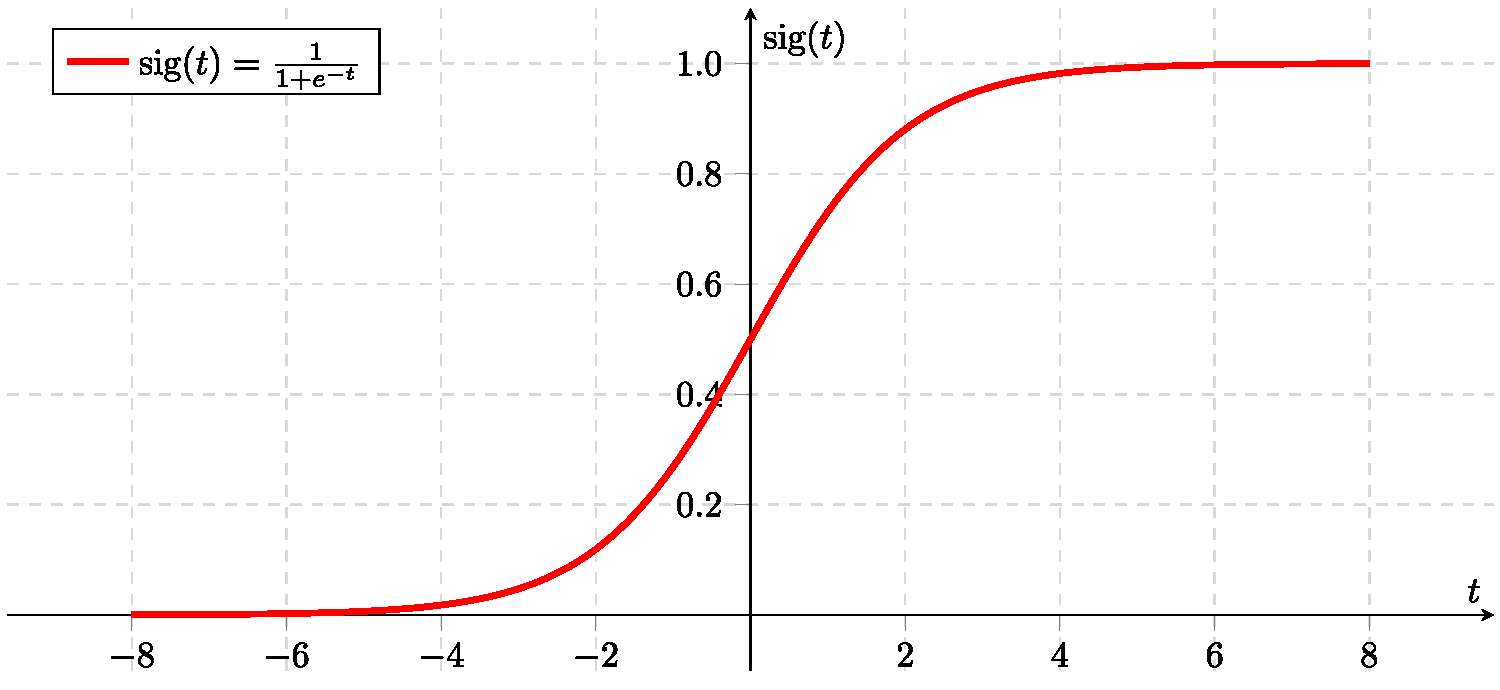
\includegraphics[width=0.45\textwidth]{grafiken/sigmoid}
    \caption[Die logistische Kurve: \textit{Von Martin Thoma, CC0}]{Die logistische Kurve}
    \label{fig:sigmoid}
\end{wrapfigure}
Es gibt mehrere Funktionen die dafür infrage kommen, aber die klassische Funktion um diesen Effekt zu erzielen ist die logistische Funktion $sig$ (\autoref{fig:sigmoid}).
Diese Sigmoidfunktion staucht Werte in den Bereich zwischen 0 und 1, indem die Werte für $t \to -\infty$ gegen 0 laufen und für $t \to \infty$ gegen 1 laufen.
Dazwischen verläuft der Graph der Funktion S-förmig.
Die Funktion wird durch folgenden Term beschrieben.
\begin{equation*}
    sig(t) = \frac{1}{1+e^{-t}}
\end{equation*}
Für die Aktivierungsfunktion $\varphi$ gilt im weiteren Verlauf dieser Arbeit immer $\varphi = sig$.\\
Die Aktivierungsfunktion wird auf den Wert eines Neurons (definiert durch~\eqref{eq:z}) angewendet.
Daraus ergibt sich folgende Funktion für den aktivierten Wert $a^l_n$ des $n$-ten Neurons auf Ebene $l$.
\begin{equation}
    a^l_n = \varphi(z^l_n)
    \label{eq:a}
\end{equation}
Der aktivierte Wert $a^l_n$ wird nun bei Anwendung des Feedforward-Verfahrens anstatt der gewichteten Summe $z^l_n$ genutzt.
Deshalb ändert sich~\eqref{eq:z} nun zu folgendem Ausdruck.
~\footcite{3b1b-1}
\begin{equation}
    z^l_n = \sum\limits^{N^{l-1}}_{i=1} a^{l-1}_i w^l_{n i}
    \label{eq:z-mit-a}
\end{equation}

\subsection{Biases}\label{subsec:biases}
Auch wenn Neuronen, Gewichtungen und eine Aktivierungsfunktion schon reichen damit ein KNN funktioniert, braucht es in den meisten Fällen noch mehr Variabilität.
Aus diesem Grund gibt es den sogenannten Bias (dt.~\textit{Verzerrung} oder \textit{Voreingenommenheit}).
Auch dieser besteht aus einem veränderbaren Zahlenwert, der für jedes Neuron in einem Netz unterschiedlich sein kann.
Ein Bias kann direkten Einfluss auf die Bedeutung seines Neurons nehmen, indem es den Wert direkt erhöht oder erniedrigt.
Dies macht das Netz anpassungsfähiger, was beim Trainieren (siehe \autoref{sec:training}) des Netzes helfen kann.
Falls sich das Neuron, zu dem der Bias gehört, nicht in der ersten Ebene des KNN befindet, wird sein Wert auf den bisherigen Wert des Neurons addiert.
Neuronen auf der ersten Ebene besitzen keine Biases, da sie die originalen Eingabewerte nur verfälschen würden und dadurch zu ungenaueren Ergebnissen beitragen würden.\\
$b^l_n$ entspricht dem Bias des $n$-ten Neurons auf Ebene $l > 1$.
Außerdem werden die Funktionen aus~\eqref{eq:z} und~\eqref{eq:a} erneut leicht angepasst und sind dadurch nun abhängig von $\overline{b}$, was alle Biases eines Netzes repräsentiert und definiert ist durch $\overline{b} = (b^2_1, b^2_2, \dots)$.
~\footcite{3b1b-1}
\begin{align}
    z^l_n &= b^l_n + \sum\limits^{N^{l-1}}_{i=1}a^{l-1}_i w^l_{n i}
    \label{eq:z-neu}\\
    a^l_n &= \varphi(z^l_n)
    \label{eq:a-neu}
\end{align}

\subsection{Beispiel}\label{subsec:beispiel}
\begin{wrapfigure}{r}{0.4\textwidth}
    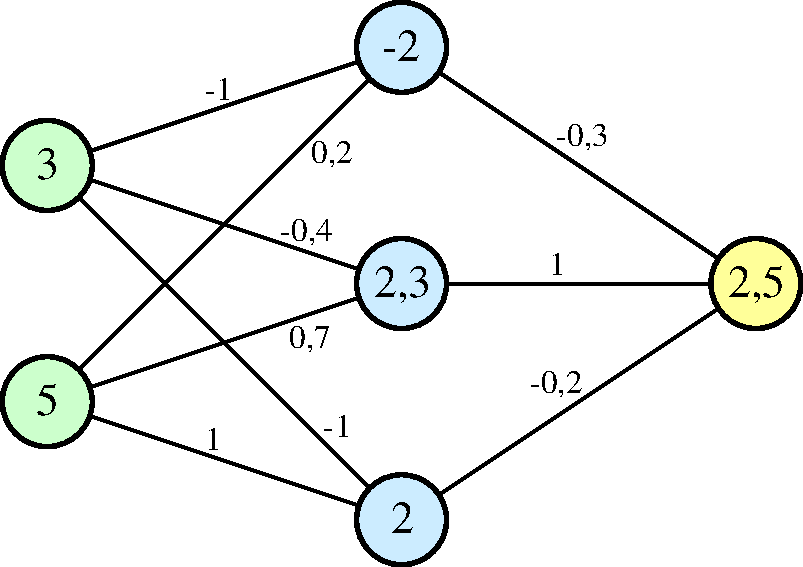
\includegraphics[width=0.4\textwidth]{grafiken/netzwerk_beispiel}
    \caption[Vereinfachte Darstellung eines künstlichen neuronalen Netzes: \textit{Eigene Grafik, erstellt in Inkscape}]{Vereinfachte Darstellung eines künstlichen neuronalen Netzes}
    \label{fig:beispiel_netz}
\end{wrapfigure}
\autoref{fig:beispiel_netz} zeigt ein Beispiel für ein KNN mit 6 Neuronen und 9 Gewichtungen, die auf 3 Ebenen verteilt sind.
Dabei sind die Eingabeneuronen grün dargestellt, das Ausgabeneuron in Gelb und die Gewichtungen als schwarze Linien.
Außerdem beinhaltet das dargestellte Netz eine verdeckte Ebene, dessen Neuronen blau eingefärbt sind.
Die Abbildung zeigt die Werte des Netzes, nachdem das Feedforward-Verfahren mit den Werten der ersten Ebene angewendet wurde.
Der Einfachheit halber wurde in der Abbildung \autoref{eq:z} verwendet, was bedeutet, dass das Feedforward-Verfahren ohne Aktivierungsfunktion und Biases angewendet wurde.